\documentclass[12pt, a4paper]{article}

\usepackage[
  margin=1in
]{geometry}

\usepackage[T1, T2A]{fontenc}
\usepackage[utf8]{inputenc}
\usepackage[russian]{babel}
\usepackage{minted}
\usepackage{hyperref}
\usepackage{tabularray}
\usepackage{amsmath}
\usepackage{float}
\usepackage{algorithm}
\usepackage{algpseudocode}
\usepackage{graphicx}

\graphicspath{ {./img/} }

\begin{document}

\begin{titlepage}
  \centering
  \textsc{Новосибирский государственный технический университет}\par
  \vspace{1mm}
  Кафедра прикладной математики\par
  \vspace{7cm}
  \textsc{Практическая работа \textnumero 4}\par
  {\huge\bfseries Решение систем нелинейных уравнений методом Ньютона\par}
  \vspace{1cm}
  {\scriptsize ФПМИ, ПМ-24\par}
  \vspace{1mm}
  {\itshape\large Параскун И., Герасименко В.\par}
  \vfill
  {\small преподаватели\par}
  \vspace{2mm}
  \textsc{Рояк М. Э., д.т.н., профессор}\par
  \vspace{1mm}
  \textsc{Задорожный А. Г., к.т.н., доцент}\par
  \vspace{1mm}
  \textsc{Леонович Д. А., ассистент}\par
  \vfill
  \large{Новосибирск, 2024}
\end{titlepage}

\newpage

\setcounter{page}{2}
\tableofcontents

\newpage

\section{Постановка задачи}
\begin{enumerate}
  \item Разработать подпрограмму решения систем нелинейных уравнений методом Ньютона.
  \item Провести тестирование подпрограммы на системах различной размерности.
  \item Провести следующие исследования метода:
    \begin{itemize}
      \item Зависимость от начального приближения;
      \item Зависимость от количества уравнений системы;
      \item Влияние взвешивания уравнений.
    \end{itemize}
  \item Разработать подпрограмму визуализации уравнений и траектории метода.
\end{enumerate}

\section{Теоретическая часть}
\noindent Метод Ньютона для систем нелинейных уравнений может быть представлен следующим образом:

\begin{align*}
  \textbf{x}^{(k)}  = \textbf{G}(\textbf{x}^{(k-1)}) 
                    = \textbf{x}^{(k-1)} - J(\textbf{x}^{(k-1)})\textbf{F}(\textbf{x}^{(k-1)})
\end{align*}
\vspace{1mm}

\noindent Организуя итерационный процесс, получаем следующий алгоритм:

\begin{algorithm}[H]
\caption{Метод Ньютона для систем нелинейных уравнений}\label{alg:newton}

\begin{algorithmic}
\State Set $\textbf{x}^{(0)}$
\State Calculate $\textbf{F}^{(0)} = \textbf{F}(\textbf{x}^{(0)})$
\State Calculate $J^{(0)} = J(\textbf{x}^{(0)})$

\For{$k=1, 2, ...$}
\State Solve $J^{(k-1)}\Delta\textbf{x}^{(k)} = -\textbf{F}^{(k-1)}$
\State Calculate $\textbf{x}^{(k)} = \textbf{x}^{(k-1)} + \Delta\textbf{x}^{(k)}$
\State Calculate $\textbf{F}^{(k)} = \textbf{F}(\textbf{x}^{(k)})$
\State Calculate $J^{(k)} = J(\textbf{x}^{(k)})$

\If{$||\Delta\textbf{x}^{(k)}|| < \varepsilon$}
\State complete
\EndIf

\EndFor
\end{algorithmic}
\end{algorithm}

\noindent В случае, если число уравнений превышает размерность системы, уравнения с минимальным абсолютным
значением исключаются.

\section{Описание разработанной программы}

\section{Описание тестирования программы}
\subsection{Тестирование на зависимость от начального приближения}
\subsubsection{Окружности соприкасаются}
\noindent Система, имеющая единственное решение:

\vspace{5mm}
\begin{figure}[H]
\centering
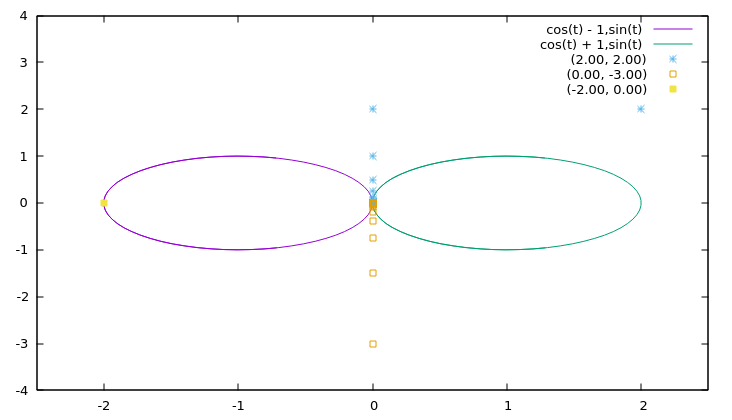
\includegraphics[scale=0.8]{1.png}
\caption{Соприкасающиеся окружности}
\end{figure}
\vspace{5mm}

\noindent с траекториями приближений \ref{t1.1} и \ref{t1.2}.

\subsubsection{Окружности пересекаются}
\noindent Система, имеющая два решения:

\vspace{5mm}
\begin{figure}[H]
\centering
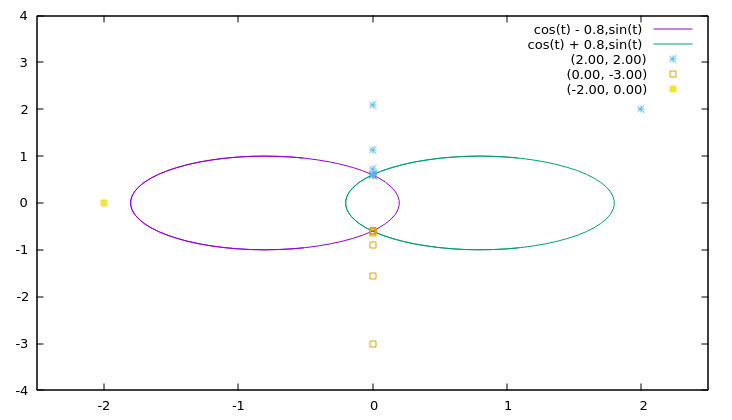
\includegraphics[scale=0.8]{2.png}
\caption{Пересекающиеся окружности}
\end{figure}
\vspace{5mm}

\noindent с траекториями приближений \ref{t2.1} и \ref{t2.2}.

\subsubsection{Окружности не пересекаются}
\noindent Система, не имеющая решений:

\vspace{5mm}
\begin{figure}[H]
\centering
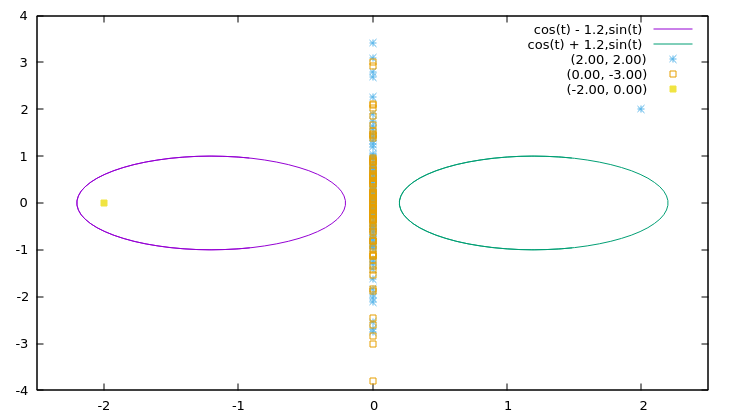
\includegraphics[scale=0.8]{3.png}
\caption{Непересекающиеся окружности}
\end{figure}
\vspace{5mm}

\noindent Начальное приближение, лежащее на горизонтальной оси, привело к аварийному завершению программы. Остальные
приближения привели к максимальному числу итераций.

\subsection{Тестирование на зависимость от количества уравнений системы}

\vspace{5mm}
\begin{figure}[H]
\centering
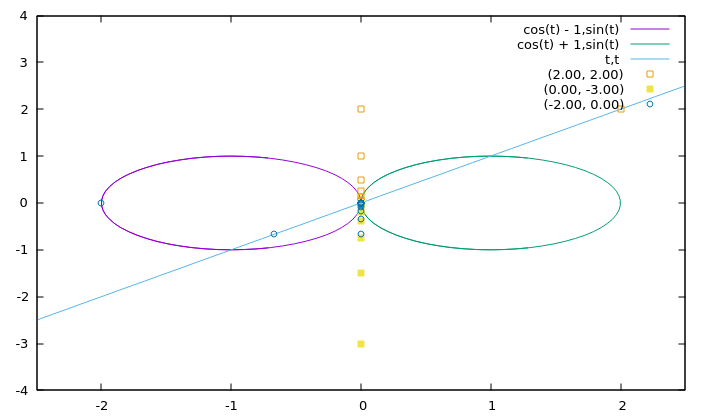
\includegraphics[scale=0.8]{4.png}
\caption{Двумерная система из трёх уравнений}
\end{figure}
\vspace{5mm}

\vspace{5mm}
\begin{figure}[H]
\centering
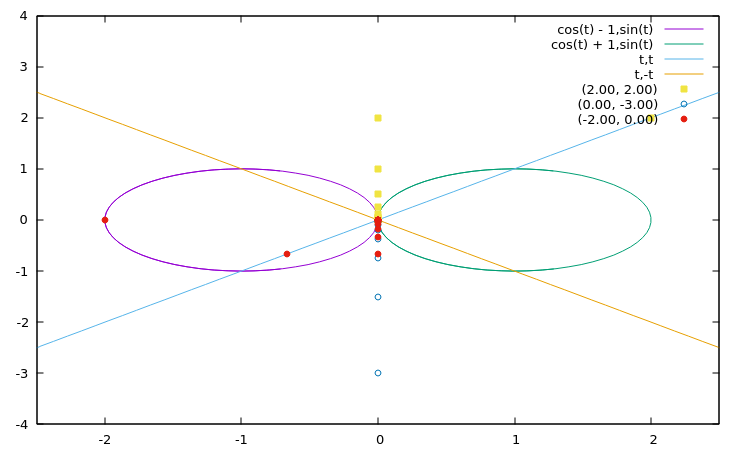
\includegraphics[scale=0.8]{5.png}
\caption{Двумерная система из четырёх уравнений}
\end{figure}
\vspace{5mm}

\subsection{Тестирование на влияние взвешивания уравнений}

\subsection{Тестирование на трёхмерной системе}
\noindent Составив систему уравнений из сферы и двух тороидов, получим:

\vspace{5mm}
\begin{figure}[H]
\centering
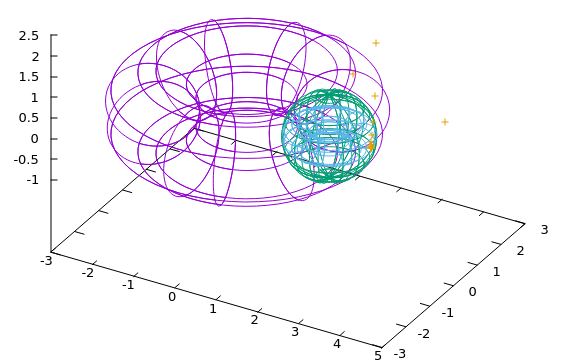
\includegraphics{10.png}
\caption{Трёхмерная система нелинейных уравнений}
\end{figure}
\vspace{5mm}

\noindent со траекторией \ref{t0}.

\section{Траектории приближений}

\begin{table}[H]
\centering
\begin{tblr}{
    width=\textwidth,
    colspec={|c|X|X|X|X|},
    rowspec={|c|ccccccccccccccccccccccccccccccc|},
}
\SetCell{c} $k$ & \SetCell{c} $x^{(k)}$ & \SetCell{c} $y^{(k)}$ & \SetCell{c} $||\Delta\textbf{x}^{(k)}||$  & \SetCell{c} $||\textbf{F}^{(k)}||$  \\
0               & 2.0000000e+00         & 2.0000000e+00         & -1.0000000e+00                            & 1.2649111e+01                       \\
1               & 1.9999558e-12         & 2.0000000e+00         & 2.0000000e+00                             & 5.6568542e+00                       \\
2               & -1.1100010e-12        & 1.0000000e+00         & 1.0000000e+00                             & 1.4142136e+00                       \\
3               & 0.0000000e+00         & 5.0000000e-01         & 5.0000000e-01                             & 3.5355339e-01                       \\
4               & 0.0000000e+00         & 2.5000000e-01         & 2.5000000e-01                             & 8.8388348e-02                       \\
5               & 0.0000000e+00         & 1.2500000e-01         & 1.2500000e-01                             & 2.2097087e-02                       \\
6               & 0.0000000e+00         & 6.2500000e-02         & 6.2500000e-02                             & 5.5242717e-03                       \\
7               & 0.0000000e+00         & 3.1250000e-02         & 3.1250000e-02                             & 1.3810679e-03                       \\
8               & 0.0000000e+00         & 1.5625000e-02         & 1.5625000e-02                             & 3.4526698e-04                       \\
9               & 0.0000000e+00         & 7.8125000e-03         & 7.8125000e-03                             & 8.6316746e-05                       \\
10              & 0.0000000e+00         & 3.9062500e-03         & 3.9062500e-03                             & 2.1579186e-05                       \\
11              & 0.0000000e+00         & 1.9531250e-03         & 1.9531250e-03                             & 5.3947966e-06                       \\
12              & 0.0000000e+00         & 9.7656250e-04         & 9.7656250e-04                             & 1.3486992e-06                       \\
13              & 0.0000000e+00         & 4.8828125e-04         & 4.8828125e-04                             & 3.3717479e-07                       \\
14              & 0.0000000e+00         & 2.4414062e-04         & 2.4414063e-04                             & 8.4293697e-08                       \\
15              & 0.0000000e+00         & 1.2207031e-04         & 1.2207031e-04                             & 2.1073424e-08                       \\
16              & 0.0000000e+00         & 6.1035156e-05         & 6.1035156e-05                             & 5.2683561e-09                       \\
17              & 0.0000000e+00         & 3.0517578e-05         & 3.0517578e-05                             & 1.3170890e-09                       \\
18              & 0.0000000e+00         & 1.5258789e-05         & 1.5258789e-05                             & 3.2927225e-10                       \\
19              & 0.0000000e+00         & 7.6293946e-06         & 7.6293944e-06                             & 8.2318063e-11                       \\
20              & 0.0000000e+00         & 3.8146972e-06         & 3.8146974e-06                             & 2.0579516e-11                       \\
21              & 0.0000000e+00         & 1.9073487e-06         & 1.9073485e-06                             & 5.1448790e-12                       \\
22              & 0.0000000e+00         & 9.5367440e-07         & 9.5367427e-07                             & 1.2862197e-12                       \\
23              & 0.0000000e+00         & 4.7683727e-07         & 4.7683714e-07                             & 3.2155494e-13                       \\
24              & 0.0000000e+00         & 2.3841884e-07         & 2.3841843e-07                             & 8.0388734e-14                       \\
25              & 0.0000000e+00         & 1.1920963e-07         & 1.1920921e-07                             & 2.0097183e-14                       \\
26              & 0.0000000e+00         & 5.9605157e-08         & 5.9604468e-08                             & 5.0242959e-15                       \\
27              & 0.0000000e+00         & 2.9803061e-08         & 2.9802095e-08                             & 1.2560740e-15                       \\
28              & 0.0000000e+00         & 1.4902152e-08         & 1.4900909e-08                             & 3.1401849e-16                       \\
29              & 0.0000000e+00         & 7.4519754e-09         & 7.4501769e-09                             & 0.0000000e+00                       \\
30              & 0.0000000e+00         & 7.4519754e-09         & 0.0000000e+00                             & 0.0000000e+00
\end{tblr}
\caption{Траектория приближений для соприкасающихся окружностей (2, 2)} \label{t1.1}
\end{table}

\begin{table}[H]
\centering
\begin{tblr}{
    width=\textwidth,
    colspec={|c|X|X|X|X|},
    rowspec={|c|ccccccccccccccccccccccccccccccc|},
}
\SetCell{c} $k$ & \SetCell{c} $x^{(k)}$ & \SetCell{c} $y^{(k)}$ & \SetCell{c} $||\Delta\textbf{x}^{(k)}||$  & \SetCell{c} $||\textbf{F}^{(k)}||$  \\
0               & 0.0000000e+00         & -3.0000000e+00        & -1.0000000e+00                            & 1.2727922e+01                       \\
1               & -3.3306691e-12        & -1.5000000e+00        & 1.5000000e+00                             & 3.1819805e+00                       \\
2               & -2.2204460e-16        & -7.5000000e-01        & 7.5000000e-01                             & 7.9549513e-01                       \\
3               & 0.0000000e+00         & -3.7500000e-01        & 3.7500000e-01                             & 1.9887378e-01                       \\
4               & 0.0000000e+00         & -1.8750000e-01        & 1.8750000e-01                             & 4.9718446e-02                       \\
5               & 0.0000000e+00         & -9.3750000e-02        & 9.3750000e-02                             & 1.2429611e-02                       \\
6               & 0.0000000e+00         & -4.6875000e-02        & 4.6875000e-02                             & 3.1074028e-03                       \\
7               & 0.0000000e+00         & -2.3437500e-02        & 2.3437500e-02                             & 7.7685071e-04                       \\
8               & 0.0000000e+00         & -1.1718750e-02        & 1.1718750e-02                             & 1.9421268e-04                       \\
9               & 0.0000000e+00         & -5.8593750e-03        & 5.8593750e-03                             & 4.8553169e-05                       \\
10              & 0.0000000e+00         & -2.9296875e-03        & 2.9296875e-03                             & 1.2138292e-05                       \\
11              & 0.0000000e+00         & -1.4648437e-03        & 1.4648437e-03                             & 3.0345731e-06                       \\
12              & 0.0000000e+00         & -7.3242187e-04        & 7.3242188e-04                             & 7.5864327e-07                       \\
13              & 0.0000000e+00         & -3.6621094e-04        & 3.6621094e-04                             & 1.8966082e-07                       \\
14              & 0.0000000e+00         & -1.8310547e-04        & 1.8310547e-04                             & 4.7415205e-08                       \\
15              & 0.0000000e+00         & -9.1552734e-05        & 9.1552734e-05                             & 1.1853801e-08                       \\
16              & 0.0000000e+00         & -4.5776367e-05        & 4.5776367e-05                             & 2.9634503e-09                       \\
17              & 0.0000000e+00         & -2.2888183e-05        & 2.2888184e-05                             & 7.4086257e-10                       \\
18              & 0.0000000e+00         & -1.1444091e-05        & 1.1444092e-05                             & 1.8521564e-10                       \\
19              & 0.0000000e+00         & -5.7220449e-06        & 5.7220462e-06                             & 4.6303911e-11                       \\
20              & 0.0000000e+00         & -2.8610215e-06        & 2.8610234e-06                             & 1.1575978e-11                       \\
21              & 0.0000000e+00         & -1.4305093e-06        & 1.4305122e-06                             & 2.8939944e-12                       \\
22              & 0.0000000e+00         & -7.1525231e-07        & 7.1525695e-07                             & 7.2349860e-13                       \\
23              & 0.0000000e+00         & -3.5762272e-07        & 3.5762959e-07                             & 1.8087465e-13                       \\
24              & 0.0000000e+00         & -1.7880627e-07        & 1.7881646e-07                             & 4.5218663e-14                       \\
25              & 0.0000000e+00         & -8.9395538e-08        & 8.9410727e-08                             & 1.1304666e-14                       \\
26              & 0.0000000e+00         & -4.4686427e-08        & 4.4709111e-08                             & 2.8261664e-15                       \\
27              & 0.0000000e+00         & -2.2326178e-08        & 2.2360248e-08                             & 6.2803698e-16                       \\
28              & 0.0000000e+00         & -1.2380630e-08        & 9.9455481e-09                             & 3.1401849e-16                       \\
29              & 0.0000000e+00         & -3.4132268e-09        & 8.9674035e-09                             & 0.0000000e+00                       \\
30              & 0.0000000e+00         & -3.4132268e-09        & 0.0000000e+00                             & 0.0000000e+00
\end{tblr}
\caption{Траектория приближений для соприкасающихся окружностей (0, -3)} \label{t1.2}
\end{table}

\begin{table}[H]
\centering
\begin{tblr}{
    width=\textwidth,
    colspec={|c|X|X|X|X|X|},
    rowspec={|c|ccccccccc|},
}
\SetCell{c} $k$ & \SetCell{c} $x^{(k)}$ & \SetCell{c} $y^{(k)}$ & \SetCell{c} $||\Delta\textbf{x}^{(k)}||$  & \SetCell{c} $||\textbf{F}^{(k)}||$  \\
0               & 2.0000000e+00         & 2.0000000e+00         & -1.0000000e+00                            & 1.1714060e+01                       \\
1               & -9.1033847e-12        & 2.0900000e+00         & 2.0020240e+00                             & 5.6683094e+00                       \\
2               & -6.6613381e-16        & 1.1311244e+00         & 9.5887560e-01                             & 1.3002879e+00                       \\
3               & -4.1633363e-17        & 7.2469589e-01         & 4.0642851e-01                             & 2.3360564e-01                       \\
4               & -4.1633363e-17        & 6.1072799e-01         & 1.1396790e-01                             & 1.8368770e-02                       \\
5               & -4.2717566e-17        & 6.0009422e-01         & 1.0633770e-02                             & 1.5991511e-04                       \\
6               & -4.2717566e-17        & 6.0000001e-01         & 9.4216087e-05                             & 1.2553509e-08                       \\
7               & -4.2717566e-17        & 6.0000000e-01         & 7.3972259e-09                             & 0.0000000e+00                       \\
8               & -4.2717566e-17        & 6.0000000e-01         & 0.0000000e+00                             & 0.0000000e+00
\end{tblr}
\caption{Траектория приближений для пересекающихся окружностей (2, 2)} \label{t2.1}
\end{table}

\begin{table}[H]
\centering
\begin{tblr}{
    width=\textwidth,
    colspec={|c|X|X|X|X|X|},
    rowspec={|c|cccccccc|},
}
\SetCell{c} $k$ & \SetCell{c} $x^{(k)}$ & \SetCell{c} $y^{(k)}$ & \SetCell{c} $||\Delta\textbf{x}^{(k)}||$  & \SetCell{c} $||\textbf{F}^{(k)}||$  \\
0               & 0.0000000e+00         & -3.0000000e+00        & -1.0000000e+00                            & 1.2218805e+01                       \\
1               & -3.9968029e-12        & -1.5600000e+00        & 1.4400000e+00                             & 2.9325132e+00                       \\
2               & 0.0000000e+00         & -8.9538462e-01        & 6.6461538e-01                             & 6.2467738e-01                       \\
3               & 0.0000000e+00         & -6.4872324e-01        & 2.4666138e-01                             & 8.6043350e-02                       \\
4               & 0.0000000e+00         & -6.0182971e-01        & 4.6893523e-02                             & 3.1098592e-03                       \\
5               & 0.0000000e+00         & -6.0000278e-01        & 1.8269308e-03                             & 4.7201871e-06                       \\
6               & 0.0000000e+00         & -6.0000000e-01        & 2.7813840e-06                             & 1.0940718e-11                       \\
7               & 0.0000000e+00         & -6.0000000e-01        & 6.4468801e-12                             & 0.0000000e+00
\end{tblr}
\caption{Траектория приближений для пересекающихся окружностей (0, -3)} \label{t2.2}
\end{table}

\begin{table}[H]
\centering
\begin{tblr}{
    width=\textwidth,
    colspec={|c|X|X|X|X|X|},
    rowspec={|c|ccccccccccccccc|},
}
\SetCell{c} $k$ & \SetCell{c} $x^{(k)}$ & \SetCell{c} $y^{(k)}$ & \SetCell{c} $z^{(k)}$ & \SetCell{c} $||\Delta\textbf{x}^{(k)}||$ & \SetCell{c} $||\textbf{F}^{(k)}||$ \\
0               & 2.0000000             & 1.0000000             & 1.0000000             & -                                        & 1.4153111                    \\
1               & 4.2360676             & 1.0000000             & 0.5000000             & 2.2912875                                & 7.7990158                    \\
2               & 2.9422403             & 0.3425763             & 2.3510197             & 2.3521201                                & 9.5347366                    \\
3               & 3.0007423             & 0.1741058             & 1.1755113             & 1.1889595                                & 2.4241266                    \\
4               & 2.9998930             & 0.0869552             & 0.5878615             & 0.5940776                                & 0.6054302                    \\
5               & 2.9999939             & 0.0434699             & 0.2939422             & 0.2971187                                & 0.1514226                    \\
6               & 2.9999996             & 0.0217339             & 0.1469726             & 0.1485682                                & 0.0378593                    \\
7               & 3.0000000             & 0.0108668             & 0.0734865             & 0.0742853                                & 0.0094651                    \\
8               & 3.0000000             & 0.0054334             & 0.0367433             & 0.0371428                                & 0.0023663                    \\
9               & 3.0000000             & 0.0027167             & 0.0183716             & 0.0185714                                & 0.0005916                    \\
10              & 3.0000000             & 0.0013583             & 0.0091858             & 0.0092857                                & 0.0001479                    \\
11              & 3.0000000             & 0.0006792             & 0.0045929             & 0.0046429                                & 0.0000370                    \\
12              & 3.0000000             & 0.0003396             & 0.0022965             & 0.0023214                                & 0.0000092                    \\
13              & 3.0000000             & 0.0001698             & 0.0011482             & 0.0011607                                & 0.0000023                    \\
14              & 3.0000000             & 0.0000849             & 0.0005741             & 0.0005804                                & 0.0000006
\end{tblr}
\caption{Траектория приближений для трёхмерной системы} \label{t0}
\end{table}

\end{document}

